\documentclass[conference]{IEEEtran}
%\IEEEoverridecommandlockouts
% The preceding line is only needed to identify funding in the first footnote. If that is unneeded, please comment it out.

\usepackage[backend=biber]{biblatex}
\addbibresource{Article.bib}
\usepackage{amsmath,amssymb,amsfonts}
\usepackage{algorithmic}
\usepackage{graphicx}
\usepackage{changepage}
\usepackage{textcomp}
\usepackage{xcolor}
\usepackage{hyperref}
\hypersetup{
	urlbordercolor=  0.2 0.8 0.72,
    pdftitle={Linking Gamification, Ludology and Pedagogy: How to Use Serious Games for Various Knowledge Domains},}
\def\BibTeX{{\rm B\kern-.05em{\sc i\kern-.025em b}\kern-.08em
    T\kern-.1667em\lower.7ex\hbox{E}\kern-.125emX}}
\begin{document}

\title{Linking Gamification, Ludology and Pedagogy: How to Use Serious Games for Various Knowledge Domains\\

}

\author{\IEEEauthorblockN{Joshua Esterhuizen}
\IEEEauthorblockA{\textit{School of Computer Science and Information Systems} \\
\textit{North-West University,}\\
Potchefstroom, South Africa \\
\href{mailto:joshua.esterhuizen27@gmail.com}{joshua.esterhuizen27@gmail.com}}
\and

\IEEEauthorblockN{Günther Drevin (Supervisor)}
\IEEEauthorblockA{\textit{School of Computer Science and Information Systems} \\
\textit{North-West University,}\\
Potchefstroom, South Africa \\
\href{mailto:Gunther.Drevin@nwu.ac.za}{Gunther.Drevin@nwu.ac.za}}

}

\maketitle

\begin{abstract}
Education as a whole has seen no major improvements for a long period of time while society has matured and grown rapidly in the same time frame. Due to this teaching and learning methods can be seen as stale to certain students. One way to solve this issue is with the implementation of some from of the technology that has developed over the years. This study looks at the possibility of adapting various domains of knowledge into digital games referred to as Serious Games. The implementation of serious games within teaching may help keep certain students engaged with the content being presented and create further interest in the topic. However, before reaching this stage the means to transform these knowledge domains into a serious games must be studied. This is done by focusing on three fields in particular, those being Gamification, Ludology and Pedagogy.
\end{abstract}

\begin{IEEEkeywords}
Education, Gamification, Knowledge Domains, Ludology, Pedagogy, Serious Games
\end{IEEEkeywords}

\section{Introduction}
Education, as it stands, is still built on a paradigm that is no longer needed in modern society. One major flaw with the current system is that it stifles the creativity and drive of some students as each level of education is largely the same and is, as such, monotonous\cite{Ackoff2008} Therefore, education requires some form of system to create an interest in learning for the students.
\\\\
Ackoff and Greenberg\cite{Ackoff2008} explain that the current traditional means of teaching are no longer as relevant as they once were as it is aimed to produce members of society that were likely to not question any fundamental aspects of how things operated. It is largely a system that focuses on teaching while disregarding learning as the last major stride in development in education was to industrialise it – having them operate efficiently like factories\cite{Ackoff2008}. It is a system that is designed to keep moving often employing a “No Child Left Behind” policy which results in almost no time for anything other than the standardised and constantly measured curriculum\cite{gibson2006games}. 
\\\\
However, with the shift into the “information age”, the requirements of the workforce have also changed. The industrial age being a time of mass-production with the emergence of various new processing technologies and the information age being characterised by the fact that information is being transmitted and generated at an ever-increasing rate due to further technological developments\cite{gibson2006games, Reigeluth1996}. The most notable changes between these ages is that the industrial age focused on conformity and compliance while initiative and diversity - where greater value is placed on each individual’s strengths and contribution to a project or organisation – is the focus of the information age\cite{Reigeluth1996}.  
\\\\
Reigeluth\cite{Reigeluth1996} continues and states that the current paradigm of instruction is not focused on learning but rather categorisation. Ackoff\cite{Ackoff1991} holds a similar viewpoint stating that there is more of a focus on teaching rather than learning. It should be noted that teaching and learning are very distinct from one another as both can take place without the other\cite{Ackoff1991}. Learning is defined as increasing one’s ability to perform an act effectively while trying to meet an objective through acquiring new knowledge whereas teaching is the process of providing this knowledge\cite{Ackoff1991}. Through this, it is clear that institutions under this paradigm aim to give learners a verbose vocabulary to speak on topics that they do not fully comprehend\cite{Ackoff1991}. 
\\\\
Due to this aforementioned paradigm shifts between the ages and in what requirements are desired by most organisations in the information age, a shift in instructional theory is also needed – one such as going from making use of passive learning through traditional teaching means to one that is centred on active learning\cite{Reigeluth1996}.
\\\\
With the recent developments in technology and the fact that technology, in general, is becoming more accessible, some institutions have adopted some forms of digital learning or supplement traditional teaching with digital assistance. Deshpande and Huang\cite{Deshpande2011} state that the current generation of students is the first to grow up with abundant access to technology. They continue to state that, on average, these students spend almost double the time playing video games as they do reading\cite{Deshpande2011}. It can be assumed that from when Deshpande and Huang’s\cite{Deshpande2011} published this work that this figure has increased as with technology and video games as industries. 
\\\\
Virvou, Katsionis and Manos\cite{Virvou2005} echo the point that computer games are popular among individuals who are in schools and as such could provide a means to deliver content in an interesting and engaging manner. 
\\\\
According to Annetta\cite{Annetta2008}, the movement for the inclusion of digital games to be used in teaching and training environments first started in 2003, two years after the field of ludology, the study of games, began to gain traction in academic literature. This initiative is what started the concept of a serious game as one that can be used in an academic sense to relay information. After this point in time, various examples of serious games were made for purely academic study purposes and had found a very large use in simulation for use as explanation aides and medical training.
\\\\
As such, the motivation behind this study is to further investigate the possibility of using video games as a means to encourage learning in teaching environments as current means of teaching may not be optimal for some individuals. This will be accomplished through studying literature in the relevant fields and identifying the instances where it is viable. The primary question aimed to be answered by this study is \textit{what qualities are required for a serious game to be effectively used in an educational environment on various topics}.
 

\section{Literature Review}
\subsection{Serious Games and Ludology}
Ludology is the formal and academic study of games and has roots in studying games through a cultural and social lens by discussing how each interacts with the so-called “spirit of play”\cite{Huizinga1949}. However, relatively recently, as early as 2001, the field has shifted and now encompasses the study of digital computer-based games as this is when the first academic peer reviewed journal on the topic was published as well as several international conferences taking place\cite{Frasca2013}. 
\\\\
As such, this study will use the definition provided by Gonzalo Frasca, “Ludology can be defined as a discipline that studies games in general, and video games in particular”\cite{Frasca2013}. Frasca\cite{Frasca2013} further elaborates on his statement that the field of ludology has a focus on discussing and understanding the individual elements of games as well as creating models to explain the various mechanics and rules of games. 
\\\\
“Serious games” were introduced as digital concepts in 2002 through the Serious Game Initiative which was spearheaded by David Rejeski and Ben Sawyer\cite{DeGloria2014}. The initial intention for serious games was for them to be used as a means of training certain tasks and skills\cite{DeGloria2014} – this was typically done through simulation type games which will be discussed in greater detail further on.
\\\\
Squire\cite{Squire2003} provides a definition for games as a simulation and states that these simulations attempt to model reality in a consistent manner usually through modelling physical or social systems through another system – which in this case would be a computer and the digital video game. There are two main types of simulations, Hi-fidelity and low fidelity. Hi-fidelity simulations attempt to model every possible interaction in a given system, phenomena or environment as accurately as possible\cite{Squire2003}. In contrast, a low fidelity simulation will make use of a fair bit of abstraction as it aims to only demonstrate a few key characteristics of the phenomena or environment\cite{Squire2003}. Games as simulations would comprise of both of these types depending on the content that it attempts to simulate.
\\\\
Virvou, Katsionis and Manos\cite{Virvou2005} mention that the endeavour to create serious games has yet to reach schools due to certain criticisms about games in general that hinders this. This is due to the fact that discussions around games by educators have largely focused on the social consequences of playing games instead of the educational potential games hold\cite{Squire2003}. Due to this the study of serious games became more theoretical and discussion-based at lower levels and more applied with actual use at higher levels. This can be seen by implementations implemented in several fields including medical rehabilitation, ecological studies, learning languages and business studies\cite{Burke2009, Costanza2014, Ranalli2008, Tao2009}. These types of games have already had an impact on the military, medical and higher business education fields early in their conception and this trend continues to this day with most serious games being used within the medical fields specifically\cite{Annetta2008, DeGloria2014}. However, there were attempts to use serious games, as simulations, within physics and engineering\cite{Deshpande2011}.
\\\\
Deshpande and Huang\cite{Deshpande2011} describe the use of games as a means of simulation for specific sections of work in physics and engineering courses as an addition to traditional teaching as it provides a relatively simple way to demonstrate certain phenomena. As such these authors discuss the simulation aspect of games rather than the narrative as when dealing with a simulation digital game it typical lacks most narrative elements in the traditional sense\cite{Deshpande2011}.

\subsection{A Pedagogical Approach}
Pedagogy is the filed that deals with the transferal of knowledge in an educational environment through several lenses such as social, political and cultural\cite{Li2012}. As such it encompasses the fields and discussions of instructional design and theory as well as any learning theories – of which several are particularly useful to this study.
\\\\
Learning by doing functions on the principle that skills can be improved through practice and self-perfection on a particular topic or knowledge base\cite{Fisch2009}. This means of instruction has become increasingly popular amongst companies where they are able to make use of “on the job” training as it allows for a person to be productive immediately as well as become more proficient at tasks gradually\cite{Fisch2009}. 
\\\\
The learning by teaching method works under the assumption that learners are able to increase their understanding of a certain topic by teaching it to other learners\cite{Fisch2009}. This method of learning has garnered more usage recently as it is a viable means of learning in environments with too few teachers or instructors and increases the overall learning process\cite{Fisch2009}. Learning methods that place the learner in control are very flexible and as such can be incorporated when attempting to teach various and different fields or subjects\cite{Ackoff1991}. 
\\\\
Gibson et al.\cite{gibson2006games} list and summarise several learning and instructional design theories that have the potential to be applied to a game used for learning. This study will, however, only look at Merrill’s First Principles of Instruction as it is the most recent of the ones depicted  and is one that is very expansive and as such can be used in a variety of manners\cite{gibson2006games}.
\\\\
Before discussing the principles that the name refers to in this theory, Merrill\cite{Merrill2002} provides a few definitions for the terms made use of. A principle in this context is a relationship that is always true regardless of the environment it is applied within – this being the driving factor for deciding to make use of this theory\cite{Merrill2002}. A practice is any instructional activity\cite{Merrill2002}. A program is a means of instruction that makes use of several practices\cite{Merrill2002}. Merrill\cite{Merrill2002} states that the first principles described are able to be implemented in any instructional system or environment as they are “design-oriented” and as such relate more to creating learning environments rather than describing the means of knowledge transfer. Each of the following principles is also accompanied by three “corollaries” each of which Merrill\cite{Merrill2002} likewise explains.
\\\\
The first principle of Merrill’s First Principles of Instruction is that the learning is problem centred. This principle describes three corollaries, the first of which being “Show Task” which states that learners should be shown the types of problems they will be solving or will be able to solve with the knowledge that they attain\cite{Merrill2002}. The next is the “Task Level” which explains that the problems presented should keep learners engaged due to the complexity and not just the action of solving it\cite{Merrill2002}. The last corollary, “Problem Progression” describes that the problems presented should have some form of increasing complexity while still being comparable to the previous iteration of the type of problem\cite{Merrill2002}.
\\\\
The second principle is Activation which means that learning happens whenever previous experiences are used\cite{Merrill2002}. The first corollary, “Previous Experience”, states that the learning process is enhanced when a learner is able to draw upon relevant past experiences and apply the associate knowledge as a foundation for new knowledge\cite{Merrill2002}. “New Knowledge” is the second and explains that learners should be provided with a relevant experience as an additional foundation to add to their knowledge base\cite{Merrill2002}. The last corollary is “Structure” and details that learners should be encouraged to organise new knowledge according to some relevant structure\cite{Merrill2002}.
\\\\
The third principle, Demonstration, proposes that learning takes place when the activities that are undertaken impart the knowledge instead of stating the information\cite{Merrill2002}. “Demonstration Consistency” explains that any examples or visualisation should be kept in line with the original learning goals\cite{Merrill2002}. The next is “Learner Guidance” and states that learners should be shown where the relevant information for problems can be found be it in the form of comparative examples or various representation of one source\cite{Merrill2002}. “Relevant Media” explains that when media is used as a means of demonstration, different types can be used provided that they do not fight for a learner’s attention\cite{Merrill2002}.
\\\\
The fourth principle is Application which states that learning takes place when learners actively solve problems with the new knowledge they have acquired\cite{Merrill2002}. “Practice Consistency” is similar to Demonstration consistency but with a focus on the application of knowledge\cite{Merrill2002}. “Diminishing Coaching” is where the learners are provided with relevant feedback, but it is slowly lessened over time\cite{Merrill2002}. It is also important that the problems provided to learners for practice have a good variety, as explained as “Varied Problems”\cite{Merrill2002}.
\\\\
The fifth, and final, principle is Integration which is when the knowledge a learner has acquired is used by them in their everyday life\cite{Merrill2002}. The first corollary, “Watch Me”, explains that learners are provided to showcase the new knowledge or skill they have acquired\cite{Merrill2002}. “Reflection” deals with giving learners time to be able to debate with others on the topic involved\cite{Merrill2002}. Lastly, “Creation” states that learners should be able to make use of their new knowledge or skill in some personal capacity\cite{Merrill2002}.

\begin{figure}[htbp]
\centerline{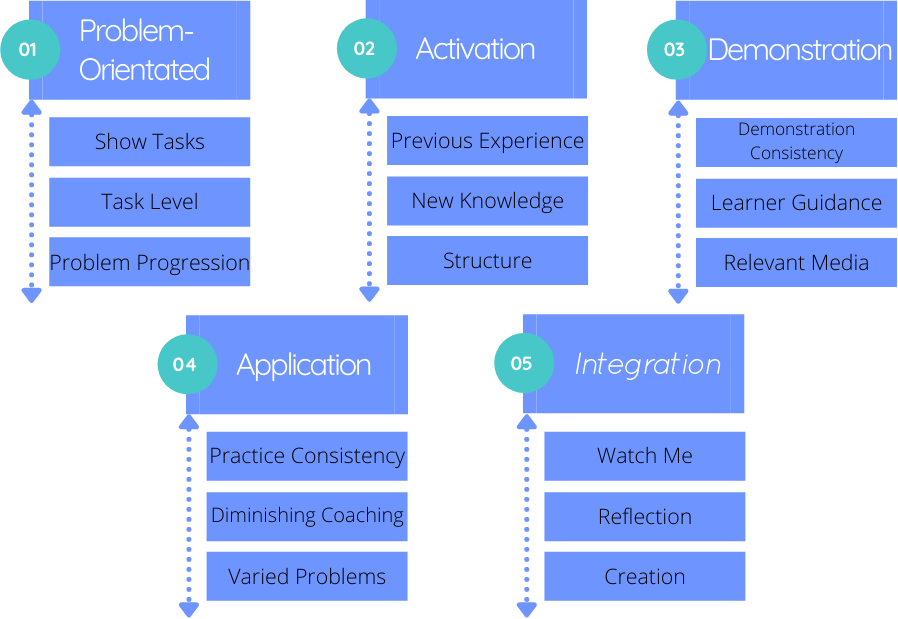
\includegraphics[scale=0.37]{merrill2.png}}
\caption{Own Image summarising Merrill's First Principles}
\label{fig}
\end{figure}

The principles and corollaries provided by Merrill\cite{Merrill2002} provide an expansive and detailed structure to be used when developing any learning opportunity making it an exceptional choice to adapt specifically to a digital game learning system.  It does, however, lack a comprehensive discussion on how to keep learners engaged with the content and, as such, the next subsection will discuss some theories pertaining to the role of motivation in learning.
\\\\
Another important factor to consider is how to keep learners engaged and motivated with the instructional material. One model for motivating learners is the ARCS Model which was developed by John Keller\cite{keller1987development} which is frequently referenced in the aforementioned field of instructional design\cite{Kapp2012a}. It is comprised of four main elements with each focusing on designing instruction in a different way\cite{Kapp2012a, keller1987development}. 
\\\\
The first of these is Attention and it is an element that is concerned with gaining and then keeping the learners’ interest. There are three main methods to accomplish this with the first being gaining attention through the use of relatable examples or surprise. The next is to create curiosity within the learners through means such as role-playing or hands-on examples. The last means to keep attention is the variability which means periodically changing the method of delivery\cite{Kapp2012a, keller1987development}.
\\\\
Relevance refers to having the content be relevant to the learner\cite{keller1987development} and Kapp\cite{Kapp2012a} mentions that this can be done through orienting the environment around achieving goals, creating a link between the motives of learners and that of the instruction means, displaying that the content is in somewhat familiar to the learners and finally developing a model of the results of learning the presented knowledge\cite{keller1987development}.
\\\\
Another element of this model, Confidence, is the expectations of success set by the learner and as such when they meet these expectations they are confident in their ability to do the work\cite{Kapp2012a, keller1987development}. This can be aided by providing learners with clear expectations and requirements upfront about the skill or knowledge. It is also helpful to provide smaller opportunities to succeed as with each success the learners will become more confident\cite{Kapp2012a, keller1987development}.
\\\\
The last element in the ARCS model is Satisfaction and is concerned with giving learners a sense of accomplishment and that the effort in the learning process has some value and weight to it\cite{Kapp2012a, keller1987development}. This can be accomplished by allowing learners to see how their new-found knowledge can be used, either through the use of a real-world demonstration or via some form of simulation\cite{Kapp2012a, keller1987development}.

\subsection{Gamification and the Knowledge Domains}
Gamification can be defined as making use of game-like mechanics, aesthetics and thinking to create motivation, solve problems and produce a more suitable learning environment\cite{Kapp2012a}. Kapp\cite{KappArticle2012} states that while gamification makes use of game elements, it only makes use of a few of them as in a gamified system, in a gamification context, learners are not constantly engaged in playing the game as there are sections of respite from this, such as video explanations. While elements such as points and achievements are found in most games, gamification strives to add more than just these to a classroom as with the absence of other elements and only points and badges, the resulting system is one that is dull\cite{KappArticle2012}. Kapp\cite{KappArticle2012} continues stating that gamification adds much more to create an interesting system such as narrative aspects and continuous feedback to learners to create and upkeep their motivation and engagement with the system.
\\\\
Gamification is often not implemented within a classroom but is rather presented to learners through some external means – such as a digital game \cite{KappArticle2012}. It should be noted, however, that a serious game can be the result of the gamification of some content but gamification does not always have to produce a serious game as a result \cite{KappArticle2012}.  
\\\\
Kapp\cite{Kapp2012a} describes various types of knowledge and how to begin developing a gamified system to effectively teach each of them. This provides the ground work for answering the question this study poses and as such allows for a more in depth discussion on how to implement serious games. These knowledge domains are described as\cite{Kapp2012a}:

\begin{itemize}
\item Declarative Knowledge is usually comprised of facts and jargon within a topic.\\
\item Conceptual Knowledge is the grouping of related information that have an underlying common descriptor.\\
\item Rules-Based Knowledge is strict statements linking concepts.\\
\item Procedural Knowledge is a progression based path to reach an outcome.\\
\item Soft Skills are general strategies for dealing with various social interactions.\\
\item Affective Knowledge deals with topics about subjective phenomena such as emotions.\\
\item Psychomotor Domain deals with making use of cognitive knowledge through physical skills (hand-eye coordination is an example of this).
\end{itemize}

One important aspect to note about these knowledge domains is that they are not mutually exclusive as one particular topic can be placed in several of them as the components of that topic may require multiple domains to be properly contained under them. 


\section{Methodology}
The following steps were taken to determine how serious games can be used for the various knowledge domains:

\begin{enumerate}
\item Literature surrounding the applicable fields was researched
\item Case studies concerning serious games was studied and similarities noted
\item Select theories that aid this process were pinpointed
\item From this research, recommendations for the knowledge domains were made
\end{enumerate}

\subsection{Sampling of Literature}
During this phase key fields of study were identifies for use in working towards the goal of this study. As discussed above, these included the fields of pedagogy (the study of instructional theory), ludology (the study of games with a focus on digital games) and gamification (the use of game-like elements to solve problems). Studying the literature in each of these fields yielded literature that is undoubtedly useful to this study as pedagogy gave insight into instructional theories used in education, ludology provided the necessary understanding of how to study games and the elements that each uses and gamification provided insight into the different knowledge domains and how to best approach each in a teaching environment in addition acting as a bridge for connecting pedagogy to the serious games in ludology. 
\\\\
The bulk of this phase was spent reading articles and identifying which would be useful for this study. It was also during this phase that select case studies were found. These case studies proved useful as each made use of different design principles and as such became another set of literature to be studied.

\subsection{Collection of Case Studies and Determine Similarities}
As case studies were accumulated, only those found that discussed - either directly in great detail or indirectly during the game's description - the design principles followed were selected to be used. Notably, many of those chosen had a focus on some form of digital and cyber security including specific mentions to phishing and social engineering\cite{Sheng2007, Dincelli2020}. 
\\\\
The following step after finding these case studies was to identify their design principles and determine the major ones that most, if not all, made use of as well as how successful the game was found to be - which is determined in the individual publication either by trails of being judged by experts.

\subsection{Pinpointing Connected Theories}
Once enough literature had been acquired and studied, the connections between each of the fields' theory and case studys' design principles were noted. This was in attempt to identify an overall pattern in the development of serious games for use particularly for educational or training purposes. This included mapping the similarities between the instructional theories to the deign principles of each case study while noting which fields of knowledge the games are a part of.  

\subsection{Extrapolate to other Knowledge Domains}
For the knowledge domains that the case studies do not directly relate to, recommendations for them will be generated out of what has been found. In addition to this, certain design principles used by the case studies can be directly applied to these domains.

\section{Findings}
As described in the methodology, a large aspect of the findings comes from the literature review conducted. However, the literature review only provided segmented information that must still be distilled. This includes making note of what instructional theory is most pertinent to this study and breaking down the case studies. It also includes a short discussion on the initial recommendations from Kapp\cite{Kapp2012a} regarding the knowledge domains.

\subsection{Helpful Instructional Theories}
This study detailed the ARCS model of motivation and Merrill's First Principles. While there are certainly others that would be helpful, these two provide sufficient knowledge to begin answering the question at hand. 
\\\\
Merrill's First Principles\cite{Merrill2002} provides a basis to begin development on a framework for serious games as it is already rooted in teaching. As such, using this theory in conjunction with the information gained from the case studies and the work done by Kapp\cite{Kapp2012a} it allows for a particular stricture to be followed.
\\\\
Similarly, the ARCS model for motivation developed by John Keller\cite{keller1987development} can be used in conjunction with Merrill's First Principles and the other findings to ensure learners are kept engaged and motivated with the games.

\subsection{Initial Knowledge Domain Recommendations}
Kapp\cite{Kapp2012a}, in addition to providing definitions of the various knowledge domains, provides some ways that each domain can be taught to best relay that particular type of knowledge. While these recommendations are derived under a gamification perspective\cite{Kapp2012a}, that can just as easily be applied for a digital game:

\begin{itemize}
\item
Games that would involve some form of sorting and matching are ideal for teaching declarative knowledge.
\item
Conceptual knowledge is beast taught through demonstrations and once again a sorting type game where the sorting is based on the common trait of the content or topic.
\item
A demonstration that displays the failure of not complying with the rules is helpful for a topic under the rules-based knowledge domain.
\item
Procedural knowledge is best taught through having the learners work through the procedure itself in some means.
\item
Soft Skills are best taught through having the learner repeatedly apply the skill in question within various scenarios.
\item
Immersing the learner within a phenomena found in the affective knowledge domain is an effective means of teaching them about it.
\item
Kapp\cite{Kapp2012a} states that observation is an ideal method of teaching the learner about a topic in the psychomotor domain.
\end{itemize}


\subsection{Case Studies and the Similarities in Design Principles}
Several case studies were examined in which some form of gamified system or serious game was developed in addition to the author(s) detailing what design principles were followed during the development process. There are three main case studies that will be focused on in this study\cite{Dincelli2020,Sheng2007,allers2021children}.
\\\\
%---------------No. 1
The first of these is titled, \textit{"Choose your own training adventure: designing a gamified SETA artefact for improving information security and privacy through interactive storytelling"} and focused on developing a gamified system to teach employees about security issues - focussing on social media and social engineering\cite{Dincelli2020}. 
\\\\
For the development of the artefact Dincelli and Chengalur-Smith\cite{Dincelli2020} made use of literature from instructional theory and gamification and as a result made use of a few key design principles. The first design principle followed is that the gamified system should make use of a \textit{story-based agent}\cite{Dincelli2020}. This means that a game should include some figure or character to guide users through the content as well as making use of story-telling in some capacity which is found to create curiosity within users\cite{Dincelli2020, Kapp2012a}. Furthermore, the use of a "choose your own adventure" style creates an interactive narrative by which the user is in control of certain decisions that change how the story plays out also improves learning\cite{Dincelli2020}. The second design principle used was that of \textit{reflection} which states that users should be given a moment of respite to dwell on what has previously been presented to them\cite{Dincelli2020,Sheng2007}.Feedback on various metrics of a users performance is also a design principle followed which allows for users to perform self evaluation\cite{Dincelli2020}. 
\\\\
The findings of this case study was that making use of a gamified system that used either visual stimuli or text were better at relaying information that traditional means and visual stimuli were better than text in terms of recognition, redintegration and ease of learning and they performed similarly in terms of recall, satisfaction and usability\cite{Dincelli2020}.
\\\\
%---------------No. 2
The next case study is titles \textit{"Anti-phishing phil: the design and evaluation of a game that teaches people not to fall for phish"} and focused on teaching people about phishing and how to avoid becoming a victim to these attacks\cite{Sheng2007}. 
\\
Sheng \textit{et al.}\cite{Sheng2007} made use of learning science theories in the games development and to refine the various iterations throughout the development process. The first two design principles discussed are \textit{reflection} and \textit{story-based agent encironment}\cite{Sheng2007}. These have already been mentioned  in the previous case study. Additionally, \textit{feedback} is also discussed in this study but specifically to how it was implemented. Anti-phishing Phil makes use of feedback both during, though displaying a short message for each choice during gameplay, and after a round of the game, through a score sheet and brief explanation of the links used\cite{Sheng2007}. 
\\\\
The next design principle followed is the \textit{procedural-conceptual principle}\cite{Sheng2007}. It should be noted that Sheng \textit{et al.}\cite{Sheng2007} mention that procedural knowledge is also referred to as declarative knowledge. A similar definition to the one Kapp\cite{Kapp2012a} provides for procedural knowledge is given and as such the definition for declarative knowledge used in this study will be the one provided by Kapp\cite{Kapp2012a}. This principle states that these two knowledge domains, conceptual and procedural, hold a mutually supportive influence over the other\cite{Sheng2007}. In practice, and thus the development of a serious game, this means that learners should be given context to the processes they are being taught as without the context they may incorrectly apply processes\cite{Sheng2007}.
\\\\
The findings of Anti-phishing phil showed that the serious game approach made users more knowledgeable on the topic and how to go about dealing with phishing\cite{Sheng2007}. While the game was a success for the most part, Sheng \textit{et al.}\cite{Sheng2007} mention that the game falls behind in one aspect - some users may become more susceptible to phishing as the game provided a fixed number of indicators to be aware of.
\\\\
%---------------No. 3
The final case study used is titled \textit{"Children’s Awareness of Digital Wellness: A Serious Games Approach"} and was targeted towards teaching children, particularly preschoolers, about digital well-being and foster cyber security awareness by means of a mobile-based serious game\cite{allers2021children}. One thing to be noted before discussing this case study is that it focused on the design and research needed for such a serious game and stated that future work could include the development and deployment of the game\cite{allers2021children}. Nonetheless, due to the level of planning done for the game as well as the positive outcome from an expert review process, this case study is still a viable option to consider. 
\\\\
While this case study\cite{allers2021children} made use of instructional theory targeted towards preschool children\cite{matthews2007,callaghan2018} some the frameworks and learning theory used can also be applied to all serious games. The first design principle followed was \textit{simplicity} as it allows a user to follow the content adequately and as such learn effectively\cite{allers2021children}. This principle is specified to the success of a awareness campaign however can also be applied to a serious game as, depending on the specific level of education, simplicity is vitally important. 
\\\\\\
The study goes on to cite Matthews \textit{et al.}\cite{matthews2007} on the ways children tend to learn. This includes:
\begin{itemize}
\item Observation
\item Listening
\item Exploring
\item Experimentation
\item Asking questions
\end{itemize}

Learning through play, such as a serious game, is an effective way to implement all of these methods\cite{allers2021children} and as such provides an additional framework targeted specifically at younger children as opposed to the previous studies\cite{Dincelli2020,Sheng2007} which were focused on adults. While this list does not provide direct principles to follow during the design process, including ways for these methods of learning to be present in a serious game should also be taken into consideration.
\\\\
In addition to the above, the study also made use of several elements identified by Callaghan \textit{et al.}\cite{callaghan2018} which are based off how young children, namely preschoolers, learn. The first of these is \textit{clear and simple goals} which is concerned with presenting a user with concise outcomes to work towards\cite{callaghan2018}. Similarly with Anti-phishing phil\cite{Sheng2007}, is the element of \textit{quality of feedback and rewards} which deals with how feedback is presented to a user - for example preschoolers may not yet be able to read and as such the feedback must be structured accordingly such as making use of simple visuals\cite{allers2021children}. The next element is \textit{Structure of the challenge} consists of setting the difficulty of tasks and changing the difficulty depending on how the user is performing\cite{callaghan2018}. This element can also be described using some of the corollaries from Merril's First Principles\cite{Merrill2002} - which will be discussed in the following section. The last element Callaghan \textit{et al.}\cite{callaghan2018} is that of \textit{Motion based learning} which describes the physical interaction a user will have with applications which in this case would be designing larger touch controls to account for a preschool child's current level of motor functions. This particular aspect is almost certainly vital when dealing with any knowledge from the psychomotor domain.
\\\\
As previously mentioned, this case study has not yet developed the serious game and as such cannot be tested by users. However, a expert review was conducted on the design of this serious game of which the outcomes were largely positive as the reviewers "found the implementations of each element satisfactory"\cite{allers2021children}.

\begin{table}[h]
\caption{Design Principles Defined by Case Study \cite{Dincelli2020,Sheng2007,allers2021children}}
\begin{adjustwidth}{-0.6cm}{}
\begin{tabular}{|c|c|c|c|}
\hline

\textbf{SETA Artefact} & \textbf{\textit{Anti-Phishing Phil}}& \textbf{\textit{Happy Hippo}} \\
\hline
Story-based	& Story-based 			& Simplicity  \\
Reflection	& Reflection			& Clear and Simple Goals  \\
Feedback	& Feedback 				& Quality of Feedback and Rewards  \\
	-		& Conceptual-Procedural	& Structure of the Challenge  \\
	-		& 		-				& Motion-based Interaction  \\
\hline

\end{tabular}
\label{tab1}
\end{adjustwidth}
\end{table}



\section{Synthesis from Research}
From the literature and case studies examined, there are several key qualities that they share among each other either under the same descriptor or with similar descriptions with different names. It is these qualities that will form the basis to answer the question posed in the beginning of this study.
\\\\
The first quality is shared amongst Merrill's First Principles\cite{Merrill2002} and two of the case studies\cite{Dincelli2020,Sheng2007}. \textit{Reflection} is then a vital quality to a serious game if intended to be used in an educational environment and is described as giving a user some time after being presented with new knowledge or a task to dwell on what they have experienced.
\\\\
The second quality a serious game should make use of is that of \textit{Feedback}. All of the case studies\cite{Dincelli2020,Sheng2007,allers2021children} mention as such and Merrill\cite{Merrill2002} refers to it under the diminishing coaching corollary. A user should be presented with feedback on how they are progressing on a given set of tasks within the game at some point and as they progress the amount of feedback should be slowly diminished. The feedback amount should also be tied to the performance of the user - increasing if they begin to struggle and decrease if not. Since feedback can take on many different forms, the type of feedback as well as the method of delivery is dependant on the topic being taught. As part of this quality, a serious game should also be designed to create an environment in which users are able to complete smaller tasks and are rewarded for these smaller successes - as per the ARCS model\cite{keller1987development}.
\\\\
Another quality that should be implemented is that the serious game should showcase and teach topics through the use of \textit{Story-telling}. The case studies\cite{Dincelli2020,Sheng2007,allers2021children} all mention the use of this and John Keller's ARCS model\cite{keller1987development}, specifically under the attention element, also states that this is a proponent of keeping users engaged. A game should then allow for a story to take place during the teaching of a topic which can also be done in several ways - such as contextually with Anti-phishing phil or as the main focus of the topic as with the SETA artefact\cite{Dincelli2020} and Happy Hippo\cite{allers2021children}. Another means to accomplish this is to make use of an agent that guides the user through the game which can be used in accordance with the Learner Guidance corollary from Merrill's First Principles\cite{Merrill2002}. 
\\\\
The last major quality a serious game should possess is that of \textit{Structuring}. This quality refers more to the content the game will deal with in terms of the instructions given as well as how the difficulty of problems could progress. It is derived from both Merrill's First Principles\cite{Merrill2002}, the ARCS model\cite{keller1987development} as well as the framework by Callaghan\cite{callaghan2018}. From the ARCS model\cite{keller1987development}, specifically Confidence, and Callaghan's\cite{callaghan2018} framework it is clear that a serious game should be structured with simple goals and clear expectations from the user and by structuring a game's instructions in this manner the user will be motivated to continue playing and therefore learning. Structuring the problems and tasks within the game should follow a similar method to how Feedback is provided - increasing the difficulty as a user gets them correct and lessening the difficulty when they are struggling to once again keep engagement with the game high. Merrill's First Principles\cite{Merrill2002} discusses this quality in several Principles and their subsequent corollaries - some of which refer to the difficulty scaling mentioned above. As such, a serious game's structure should be centred around the problems themselves - or the knowledge being taught when dealing with Affective knowledge and soft skills. The tasks given to a user should be both varied to keep the users' attention as well as be consistent in the ways the user interacts with them. This approach should keep users motivated to use the game according to the ARCS model\cite{keller1987development} as it makes use of both the Attention and Relevance elements.
\\\\
While the remaining aspects of the pedagogical theories and design principles from the case studies are also useful in the implementation of a serious game, they are specific to the content being taught and as such should be considered in greater detail if a similar game to those were to be developed.

\subsection{Recommendations for Specific Knowledge Domains}
Kapp's\cite{Kapp2012a} recommendations are a helpful starting point to how to effectively teach content relating to the knowledge domains. 
\\\\
Referring back to Squire's\cite{Squire2003} descriptions of games as simulations - both Hi-fidelity and low fidelity. These types of serious games are certainly the most useful for teaching content found in the Affective, Soft Skills and Psychomotor domains since the best means to teach these is through immersing the user in the phenomena, repeated application of skills and observation respectively\cite{Kapp2012a}. Simulation-type serious games can also be used in the other domains such as with the game used to aid in teaching physics described by Deshpande and Huang\cite{Deshpande2011}. These types of games are also the most effective means for the psychomotor domain as shown by various studies\cite{Burke2009, Costanza2014, Ranalli2008, Tao2009}.
\\\\
The remaining knowledge domains tend to have some heavy overlap depending of the topic being covered. Sheng \textit{et al.}\cite{Sheng2007} discussed the Conceptual-Procedural principle in their game's development. To reiterate, it simply states that a topic cannot be fully understood from only the procedures or context - both are needed for a deeper understanding.

\section{Limitations and Future Research}
This study made use of various fields of study as well as case studies of serious games and their design in order to answer the question posed. The current limitations of answering the question largely center around the amount of literature sourced. In terms of the fields looked at (pedagogy, ludology and gamification) these seem to be sufficient in terms of what literature can be used and as such it is the specific literature used that imposes limitations. There are many more instructional theories that could be considered and as such future research could delve into more theories and expand the knowledge base used to answer the question. Future research could also include looking at various types of games and how they could teach content in the different knowledge domains to build upon Kapp's\cite{Kapp2012a} recommendations. Another limitation comes from the case studies used. All of the main case studies discussed in this article had a focus on computer security to varying degrees. Due to this, future research could include case studies on the design, implementation or development of serious games in other fields.
\\\\
Furthermore, a more practical approach to future research could include the development of a serious game on a topic based in one of the knowledge domains mentioned. This could include the development an artefact for user testing, similarly to Anti-phishing phil\cite{Sheng2007}, based off of the findings of this study or the designing of such an artefact more in line with the "Happy Hippo" game\cite{allers2021children}.

\section{Conclusion}
This study discussed the current state of the paradigms that instructional institutions are based off of and how society has progressed and developed different needs than the systems in place currently provide. As such, research into how serious games can be used in an educational environment was conducted with specific focus on the fields of pedagogy, ludology and gamification in order to answer the question, \textit{what qualities are required for a serious game to be effectively used in an educational environment on various topics}. Through a literature review in these fields, various instructional theories were found that could be helpful to answer the question as they are able to be translated into the context of games relatively easy. Furthermore, several research papers were used as case studies to discover what design principles are typically followed in the development of serious games. This information was then used to identify what are the major qualities which a serious game should have in order to be effective in a educational environment as well as providing specific recommendations for various knowledge domains. The qualities identified were allowing for Reflection, providing Feedback, making use of Story elements and a well thought out Structuring of the game. Recommendations for the different knowledge domains were also given.
\\
\section*{Acknowledgements}
This article was part of a research project for an Honours degree and as such I would like to thank my supervisor, Günther Drevin, for their aid throughout the year as well as for the lessons on the field of ludology as well as the School of Computer Science and Information Systems at the North West University for providing this opportunity.


\printbibliography

\end{document}
